\documentclass[10pt]{beamer}
\logo{
\includegraphics[width=.05\textwidth]{logo6.png}}
  \usetheme{CambridgeUS}       % or try default, Darmstadt, Warsaw, ...
 \usecolortheme{seahorse} % or try albatross, beaver, crane, ...
  \usefonttheme{serif}    % or try default, structurebold, ...
  \setbeamertemplate{navigation symbols}{}
  \setbeamertemplate{caption}[numbered]
\usepackage{xcolor}
\usepackage{tabularx}
\usepackage{graphicx}
\usepackage{subcaption}
\usepackage{lmodern}
\usepackage[scale=2]{ccicons}
\usepackage{multirow}
\usepackage{animate}
\usepackage{listings}
\usepackage{amsmath}
\usepackage[flushleft]{threeparttable}
\usepackage[english]{babel}
\usepackage{picture}
\usepackage{tikz}
\usepackage[absolute,overlay]{textpos}
\usepackage{spot}
\definecolor{back}{RGB}{253, 250, 255}
\definecolor{points}{RGB}{94, 103, 229}
\definecolor{comp}{RGB}{35, 99, 70}
\definecolor{inc}{RGB}{191, 13, 43}
\setbeamercolor*{item}{bg=points}
\setbeamercolor*{background canvas}{bg=back}  
%\setbeamercovered{dynamic}

%\AtBeginSection[]{
%  \begin{frame}
%  \vfill
%  \centering
%  \begin{beamercolorbox}[sep=8pt,center,shadow=true,rounded=true]{title}
%    \usebeamerfont{title}\insertsectionhead\par%
%  \end{beamercolorbox}
%  \vfill
%  \end{frame}
%}
%
%\AtBeginSubsection[] % Do nothing for \subsection*
%{
%\begin{frame}
%  \vfill
%  \centering
%  \begin{beamercolorbox}[sep=8pt,center,shadow=true,rounded=true]{title}
%    \usebeamerfont{title}\insertsubsectionhead\par%
%  \end{beamercolorbox}
%  \vfill
%  \end{frame}
%}

\begin{document}

\title[]{DscoreApp: A Shiny App for the computation of the IAT D-score}
\author[]{Ottavia M. Epifania}
\institute[]{University of Padova}
\date{19\textsuperscript{th} September 2019}


\begin{frame}[plain]
  \titlepage
\end{frame}

%
%\begin{frame}
%\frametitle{Contents}
%\tableofcontents[subsectionstyle=hide]
%\end{frame}

\section{The Implicit Association Test}
\begin{frame}
\begin{table}[th!]
\centering
\caption{IAT structure.}
\begin{tabularx}{\linewidth}{llll}
\hline
Block  & Function & Left key & Right key \\ \hline
B1  & Practice & Flowers & Insects \\
B2  & Practice & Good & Bad \\
\color{comp}{B3}  & \color{comp}{Practice Mapping A} & \color{comp}{Flowers + Good} & \color{comp}{Insects + Bad} \\
\color{comp}{B4}  & \color{comp}{Test Mapping A} & \color{comp}{Flowers + Good} & \color{comp}{Insects + Bad} \\
B5  & Practice & Insects & Flowers \\
\color{inc}{B6}  & \color{inc}{Practice Mapping B} & \color{inc}{Insects + Good} & \color{inc}{Flowers} + \color{inc}{Bad}\\
\color{inc}{B7}  & \color{inc}{Test Mapping B} & \color{inc}{Insects + Good} & \color{inc}{Flowers + Bad}\\
\hline
\end{tabularx}
\end{table}
\end{frame}


\section{The D-score}
\begin{frame}

\begin{textblock*}{3.5cm}(0.7cm,1.3cm)

\begin{equation*}
D_{practice} = \frac{M_{b6} - M_{b3}}{sd_{b6,b3}}
\end{equation*}
\begin{equation*}
D_{test} = \frac{M_{b7} - M_{b4}}{sd_{b7,b4}}
\end{equation*}
\end{textblock*}

\begin{textblock*}{3.5cm}(6.7cm,1.8cm)
\begin{equation*}
D_{score} = \frac{D_{practice} + D_{test}}{2}
\end{equation*}
\end{textblock*}

\begin{textblock*}{\linewidth}(0.7cm,3.7cm)
\small
\begin{table}[th!]
\centering
\caption{\emph{D-score} algorithms.}
\begin{tabularx}{\linewidth}{llll}
\hline
\emph{D} & Error inflation & Lower tail treatment\\\hline
\emph{D-score1} & Built-in correction & No \\
\emph{D-score2} & Built-in correction & Delete trials $<$ 400 \emph{ms} \\
\emph{D-score3} & Mean (correct responses) + 2\emph{sd} & No\\
\emph{D-score4} & Mean (correct responses) + 600 \emph{ms} & No \\
\emph{D-score5} & Mean (correct responses) + 2\emph{sd} & Delete trials $<$ 400 \emph{ms}\\
\emph{D-score6} & Mean (correct responses) + 600 \emph{ms} & Delete trials $<$ 400 \emph{ms} \\
\emph{D SC-IAT} & Mean + 400\emph{ms} & Delete trials $<$ 350 \emph{ms} \\\hline
\end{tabularx}
\end{table}
\end{textblock*}
\end{frame}

\subsection{Available Options}
\begin{frame}
\begin{small}
\begin{table}[th!]
\centering
\caption{\label{tab:packages} Overview of the available options for computing the \emph{D-score}.}
\begin{tabularx}{\linewidth}{ll l ll}
\hline
  &  Open source &  Programming skills &  Multiple D-score &  Plot \\
\hline
SPSS syntaxes  & No & A bit & Yes & No \\
Inquisit scripts & No & No & No & No  \\
\texttt{IATanalytics}  & Yes & Yes & Not clear & No  \\
\texttt{IATScore}  & Yes & Yes & Not clear & No \\
\texttt{IAT} & Yes & Yes & Yes & Yes  \\
\texttt{IATScores}  & Yes & Yes & Yes  & Yes   \\
\hline
\end{tabularx}
\end{table}
\end{small}

\pause
\begin{itemize}
\item[{
\includegraphics[height=5ex]{emoji.png}}] Something Open Source, user-friendly, able to compute multiple scores
\end{itemize}


\end{frame}

\section{DscoreApp}
\begin{frame}
\begin{figure}
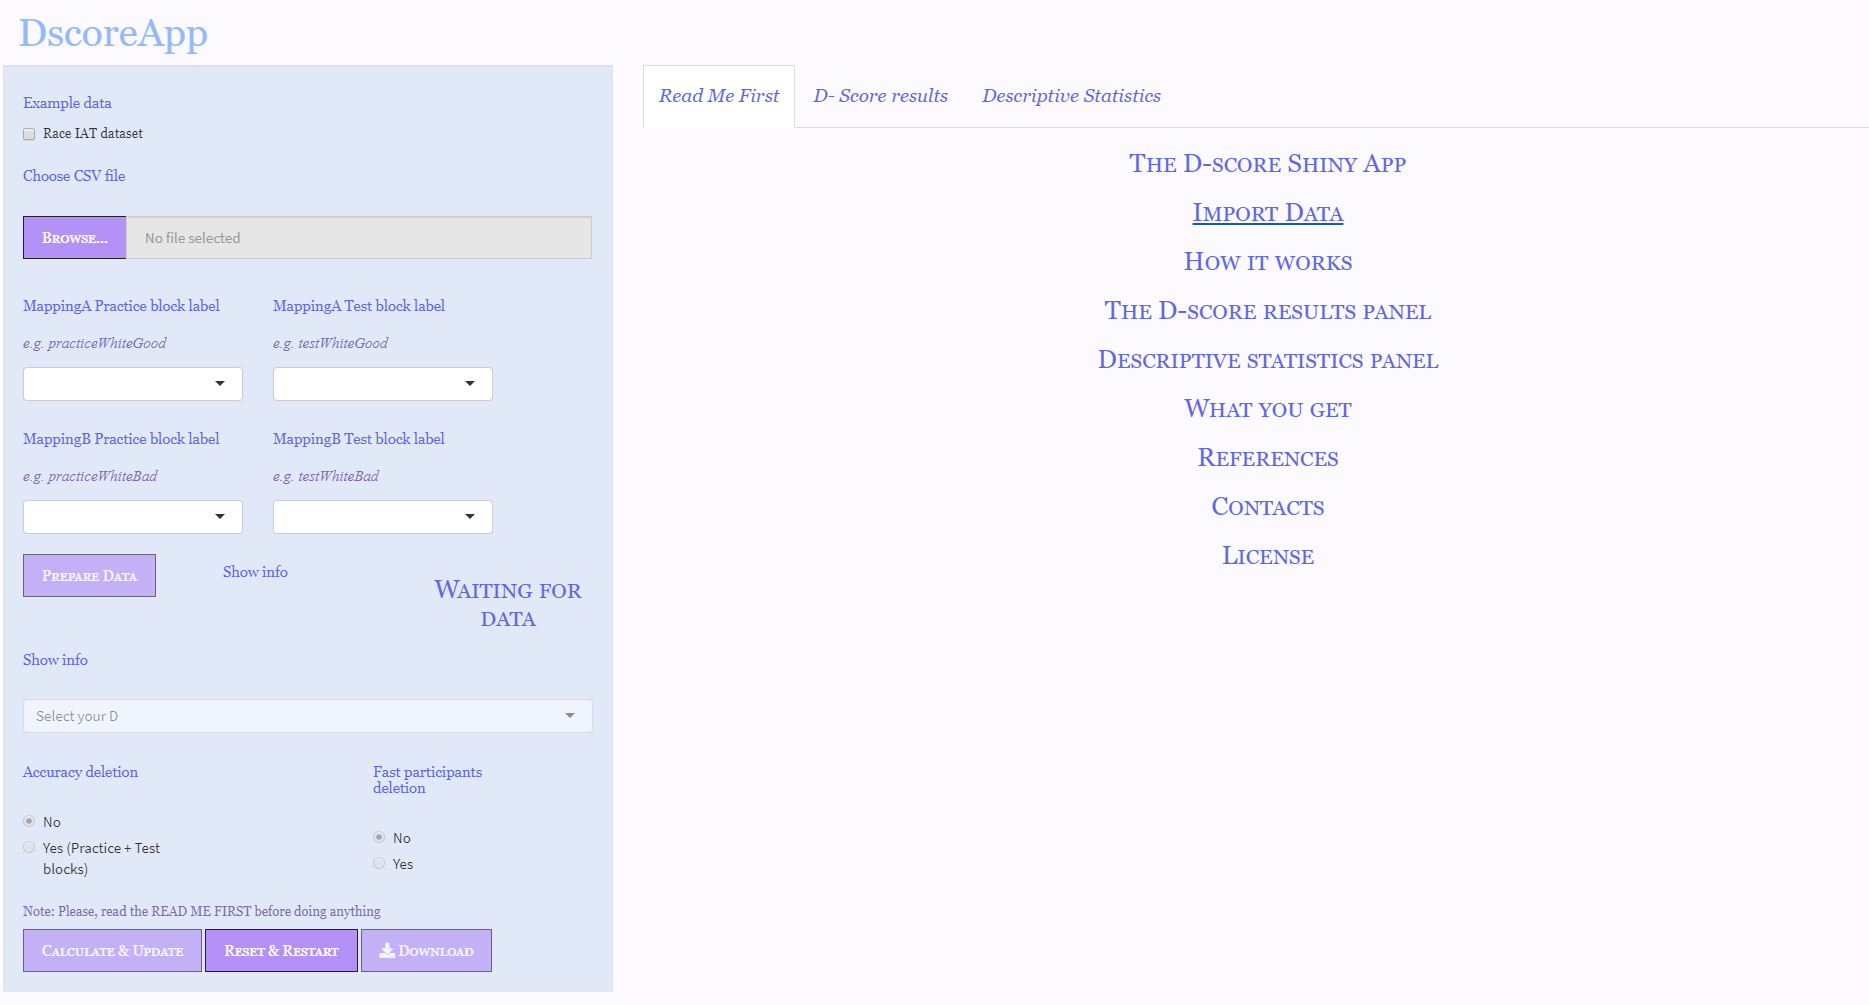
\includegraphics[width=\linewidth]{app.png}
\end{figure}

\begin{textblock*}{10cm}(3cm, 4.5cm)
{\includegraphics<2->[width=\linewidth]{details.png}}
\end{textblock*}
\end{frame}

\subsection{Upload, Prepare, and Compute}
\begin{frame}
\begin{figure}
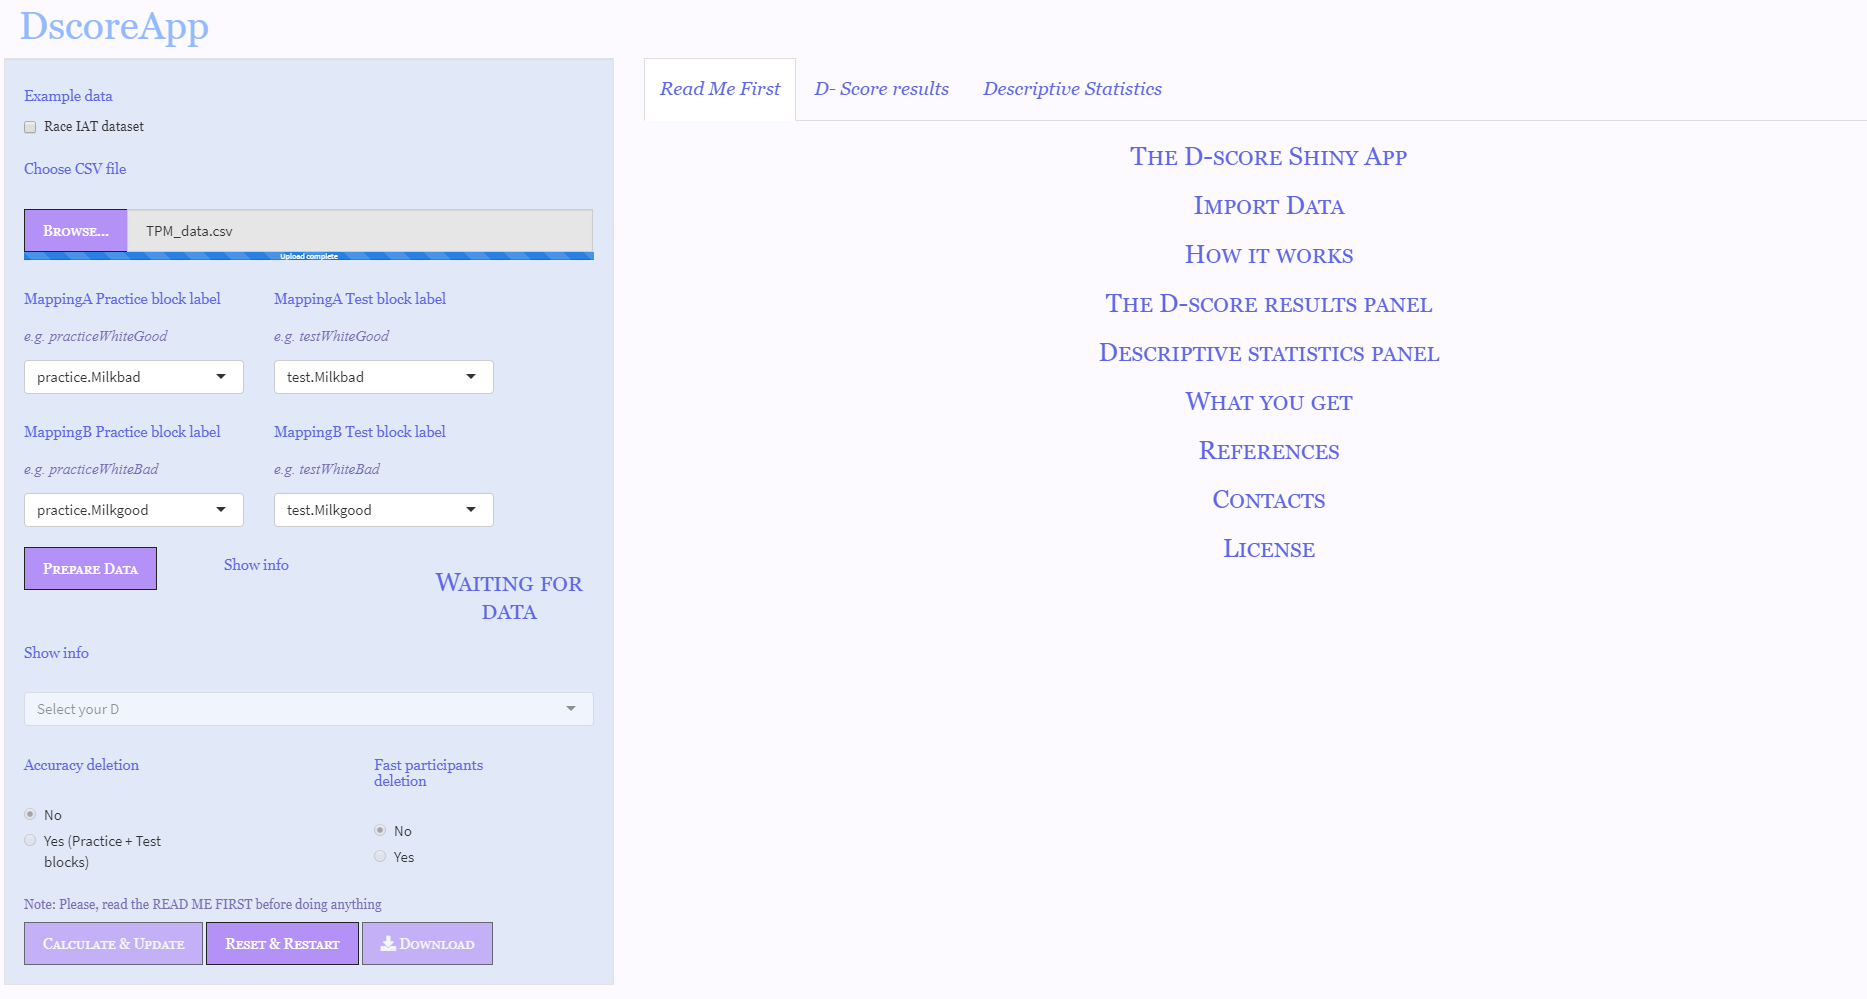
\includegraphics[width=\linewidth]{upload.png}
\end{figure}

\begin{textblock*}{10cm}(2cm, 0.5cm)
{\includegraphics<2->[width=0.5\linewidth]{select.png}}
\end{textblock*}

\begin{textblock*}{10cm}(3cm, 4.5cm)
{\includegraphics<3->[width=0.5\linewidth]{compute.png}}
\end{textblock*}
\end{frame}

\subsection{Plot} 
\begin{frame}
\begin{figure}
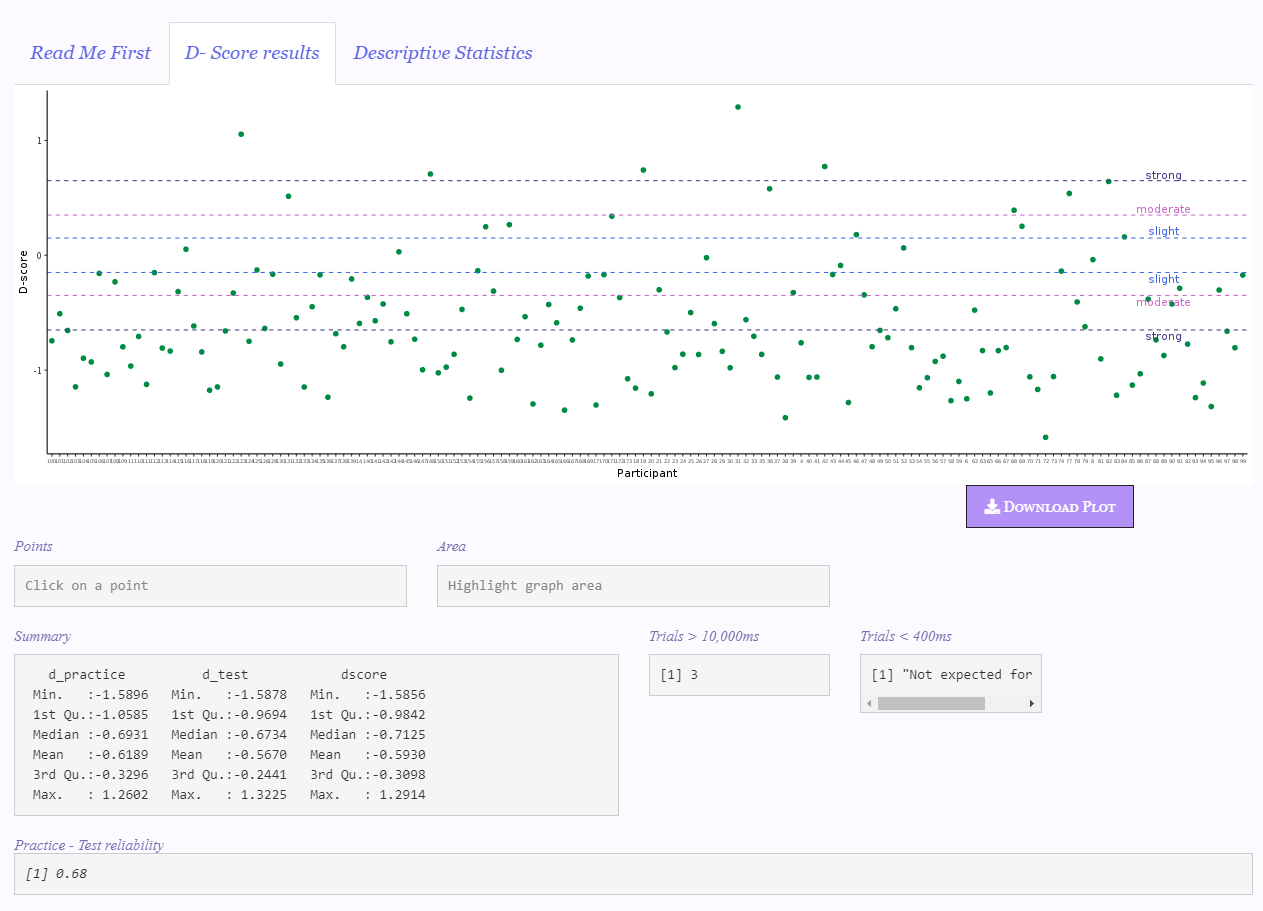
\includegraphics[width=\linewidth]{results.png}
\end{figure}

\begin{textblock*}{10cm}(2cm, 0.8cm)
{\includegraphics<2->[width=0.8\linewidth]{points.png}}
\end{textblock*}

\begin{textblock*}{10cm}(3cm, 4.5cm)
{\includegraphics<3->[width=0.8\linewidth]{area.png}}
\end{textblock*}
\end{frame}

\begin{frame}[plain]
\begin{center}
\vspace{1cm}
  \texttt{Thanks!}

\vspace{1cm}

\begin{itemize}
\item[{
\includegraphics[height=3ex]{logo6.png}}] \url{http://fisppa.psy.unipd.it/DscoreApp/}
\item[{\small
\includegraphics[height=2.8ex]{download.png}}] \url{{otta.epifania@gmail.com}}
\item[{\small
\includegraphics[height=2.8ex]{github.png}}] \href{https://github.com/OttaviaE}{@OttaviaE}
\item[{\small
\includegraphics[height=2.8ex]{twitter.png}}] \href{https://twitter.com/ExeOttavia}{@ExeOttavia}
\end{itemize}
\end{center}

\end{frame}
\end{document}